%%%%%%%%%%%%%%%%%%%%%%%%%%%%%%%%%%%%%%%%%%%%%%%%%%%%%
%			CELÝ ZPĚVNÍK v. 18.09  					%
%%%%%%%%%%%%%%%%%%%%%%%%%%%%%%%%%%%%%%%%%%%%%%%%%%%%%
% Toto je hlavní soubor zpěvníku, z kterého lze 
% kompilovat celý zpěvník se všemi písničkami.
%%%%%%%%%%%%%%%%%%%%%%%%%%%%%%%%%%%%%%%%%%%%%%%%%%%%%
%			Jak kompilovat celý zpěvník?			%
%%%%%%%%%%%%%%%%%%%%%%%%%%%%%%%%%%%%%%%%%%%%%%%%%%%%%
% Přidání nové písničky probíhá tak, že:
% 1. Napíšete .tex soubor s textem písničky a akordy 
% a soubor vložíte do ../songy
%	a) Soubor se píše podle pravidel napsaných 
%	   v souboru ../Generator/generator.tex
%	b) V souboru ../Generator/generator.tex
%	   se soubor také kompiluje samostatně 
%      pro kontrolu.
% 2. Písnička se přidá na místě označeném kódem 
%    PRIDAVANI (ctrl+f a dá se to najít). Přidáte 
%    ji vložením následujícího řádku podle abecedy: 
%    \addcontentsline{toc}{section}{[ZDE NAPIŠ NÁZEV PÍSNIČKY]}\input{../songy/[ZDROJOVÝ SOUBOR PÍSNIČKY].tex}\newpage
% 3. Výsledek s zobrazí po kompilaci DVAKRÁT 
%    za sebou (kvůli toc).
% (4.) Předmluva se upravuje na místě PŘEDMLUVA.
% (5.) Cover obrázek: PŘEBAL1
% (6.) Watermark: VODOZNAK
% (7.) Seznam všech akordů: PŘEHLED
%%%%%%%%%%%%%%%%%%%%%%%%%%%%%%%%%%%%%%%%%%%%%%%%%%%%%
%			Jak kompilovat jednotlivé písně?        %
%%%%%%%%%%%%%%%%%%%%%%%%%%%%%%%%%%%%%%%%%%%%%%%%%%%%%
%	1. Více návodu je k tomuto napsáno v souboru 
%      ../Generator/generator. 
%%%%%%%%%%%%%%%%%%%%%%%%%%%%%%%%%%%%%%%%%%%%%%%%%%%%%
%			Jak psát soubory songů?                 %
%%%%%%%%%%%%%%%%%%%%%%%%%%%%%%%%%%%%%%%%%%%%%%%%%%%%%
%	1. Více návodu je k tomuto napsáno v souboru 
%      ../songy/00Songtemplate. 
%%%%%%%%%%%%%%%%%%%%%%%%%%%%%%%%%%%%%%%%%%%%%%%%%%%%%

\documentclass[openany,12pt]{memoir}
\usepackage[utf8]{inputenc}
\usepackage[czech]{babel}
\usepackage[T1]{fontenc}
\usepackage[top=1.5cm, bottom=2cm, left=2cm, right=2cm]{geometry}  % --> NASTAVENÍ OKRAJŮ
\usepackage{fancyhdr}
\usepackage{graphicx}
\usepackage{xwatermark}
\usepackage{xcolor}
\usepackage{changepage}
\usepackage{pdfpages}
\usepackage{lettrine}
\usepackage{indentfirst}  %Důležité pro formátování

%%%%%%%%%%%%%%%%%%%%%%%%%%%%%%%%%%%%%%
%  FONT                              %
%%%%%%%%%%%%%%%%%%%%%%%%%%%%%%%%%%%%%%
\usepackage{amssymb}
\usepackage{tgschola}



%%%%%% Package na zpěvník
\usepackage[full]{leadsheets}%http://mirrors.nic.cz/tex-archive/macros/latex/contrib/leadsheets/leadsheets_en.pdf   --> dokumentace	
\definesongtitletemplate{empty}{} 
\setchords{
format = \bfseries \sffamily,   %tučné akordy
minor = {mi},% 
input-notation = {german},%
output-notation = {german}%
}
\definesongtitletemplate{empty}{} 

\newlength{\drop}
% VODOZNAK
\newwatermark[pages=3-,color=red!50,angle=0,scale=2, xpos=0,ypos=0]{
\includegraphics[width=5cm]{obr/pozadi2.jpg}} %--> dvojka na pozadí


%%%%%%%%%%%%%%%%%%%%%%%%%%%%%%%%%%%%%%%%%%%%%%%%%%
%		 Vlastní příkazy
\newcounter{Slokočet}   %Automatické číslování slok
\newcommand{\mezera}{
\phantom{.}

}   %Horizontální odsazení slok (poněkud blbě zadefinovaný, ale jinak se formát rozbije jako wtf prostě)
\newcommand{\stred}{5.2cm}   %%% Na zarovnání slok doprostřed, pozn. automatičtější zarovnávání na střed nejde
\newcommand{\carka}{,\:}
\newcommand{\m}[1]{\color{white}{#1}}  %Pro akordy
\newcommand{\ap}{'}	%Pro apostrof
\newcommand{\elipsa}{\kern\fontdimen3\font} %Příkaz pro lepší zacházení s výpustkami (=...); je to vpodstatě jen mezera mezi tečkama výpustky
\newcommand{\pindent}{17.62482 pt} %Správná velikost \parindentu u layoutu se dvěma minipageama
\newcommand{\predtitle}{\huge}
\newcommand{\mezisloupci}{\phantom{TT}} %Místo mezi dvěma sloupci na jedné stránce
\newcommand{\z}{\hspace*{\fill}\null}

%%% Možné velikosti písem 
\newcommand{\normalni}{\normalsize}
\newcommand{\velky}{\fontsize{14.4}{15}\selectfont}
\newcommand{\vetsi}{\fontsize{15}{16}\selectfont}
\newcommand{\nejvetsi}{\fontsize{16}{17}\selectfont}
\newcommand{\nejnejvetsi}{\fontsize{17}{19}\selectfont}

%%% Stará definice sloky spoléhající na indenty
%\newlength{\pismeno}
%\settowidth{\pismeno}{x} %Tohle není moc ideální velikost, ale funguje
%\newif\ifslokavelka
%\slokavelkafalse
%\newcommand{\sloka}{
%\ifnum \value{Slokočet}>8  %Pokud je sloka dvouciferná
%\mezera \noindent \addtocounter{Slokočet}{1} \hspace*{-\pismeno}\arabic{Slokočet}.
%\else %Pokud jen jednociferná
%\mezera \noindent \addtocounter{Slokočet}{1} \arabic{Slokočet}. 
%\fi
%} 	%sloka, která se automaticky čísluje

\newcommand{\distanc}{\:}  %Vzdálenost čísla sloky před slokou
\newlength{\delkaargumentu}
%%% Sloka s automatickým číslováním
\newcommand{\sloka}{%
\addtocounter{Slokočet}{1}% Zvýší se o 1 počet slok
\mezera%  Sloka se odsadí vertikálně
\settowidth{\delkaargumentu}{\arabic{Slokočet}.\distanc}% Zde se určí délka odsazení 
\hspace*{-\delkaargumentu}%
\arabic{Slokočet}.\distanc%
\ignorespaces% Aby nevznikaly zbytečné mezery
}


%%% Sloka s vlastním argumentem
\newcommand{\ssloka}[1]{%     
\settowidth{\delkaargumentu}{#1\distanc}
\mezera%
\hspace*{-\delkaargumentu}%
#1\distanc%
\ignorespaces%
}  

%%% Refrén
\newcommand{\refren}[1][0]{%  Nepovinný argument sděluje, kolikátý refrén toto je, bez argumentu se vytiskne pouze refrén
\ifnum #1>0 %Pokud nepovinný argument existuje
\mezera%
\settowidth{\delkaargumentu}{\textbf{R$_{\text{#1}}$:}\distanc}%
\hspace*{-\delkaargumentu}%
\textbf{R$_{\text{#1}}$:}\distanc%
\ignorespaces%
\else %Pokud nepovinný argument neexistuje
\mezera%
\settowidth{\delkaargumentu}{\textbf{R:}\distanc}%
\hspace*{-\delkaargumentu}%
\textbf{R:}\distanc%
\ignorespaces%
\fi
}

\newcommand{\predehra}{\ssloka{\textbf{Předehra:}}}


\addto\captionsczech{\renewcommand{\contentsname}{Seznam písní}}

%%%%%%%%%%%%%%%%%%%%%%%%%%%%%%%%%%%%
%    FORMÁTOVÁNÍ                   %
%%%%%%%%%%%%%%%%%%%%%%%%%%%%%%%%%%%%

%%% Vlevo zarovnaný text s blokem zarovnaným na střed
\usepackage{varwidth}% http://ctan.org/pkg/varwidth
\newenvironment{centerjustified}{%
  \begin{center} % so the minipage is centered
  \begin{varwidth}[t]{\textwidth}	
  \raggedright % so the minipage's text is left justified
  \setlength{\parindent}{\pindent}
}{%
  \end{varwidth}
  \end{center}
}


\usepackage{hyperref} %Musí být načteno jako poslední package
\begin{document}
\sffamily %Sans-serif font vypadá lépe
\velky   %Minimální čitelná velikost


\renewcommand{\abstractname}{\vspace{-\baselineskip}} %Aby nad úvodním textem nebyl nápis ,,Abstract''


%Kompilovat dvakrát, aby se updatnula TOC

\setcounter{page}{0}
\pagestyle{empty}
%%%%%%%%%%%% PŘEBAL1 %%%%%%%%%%%%%%%%%%
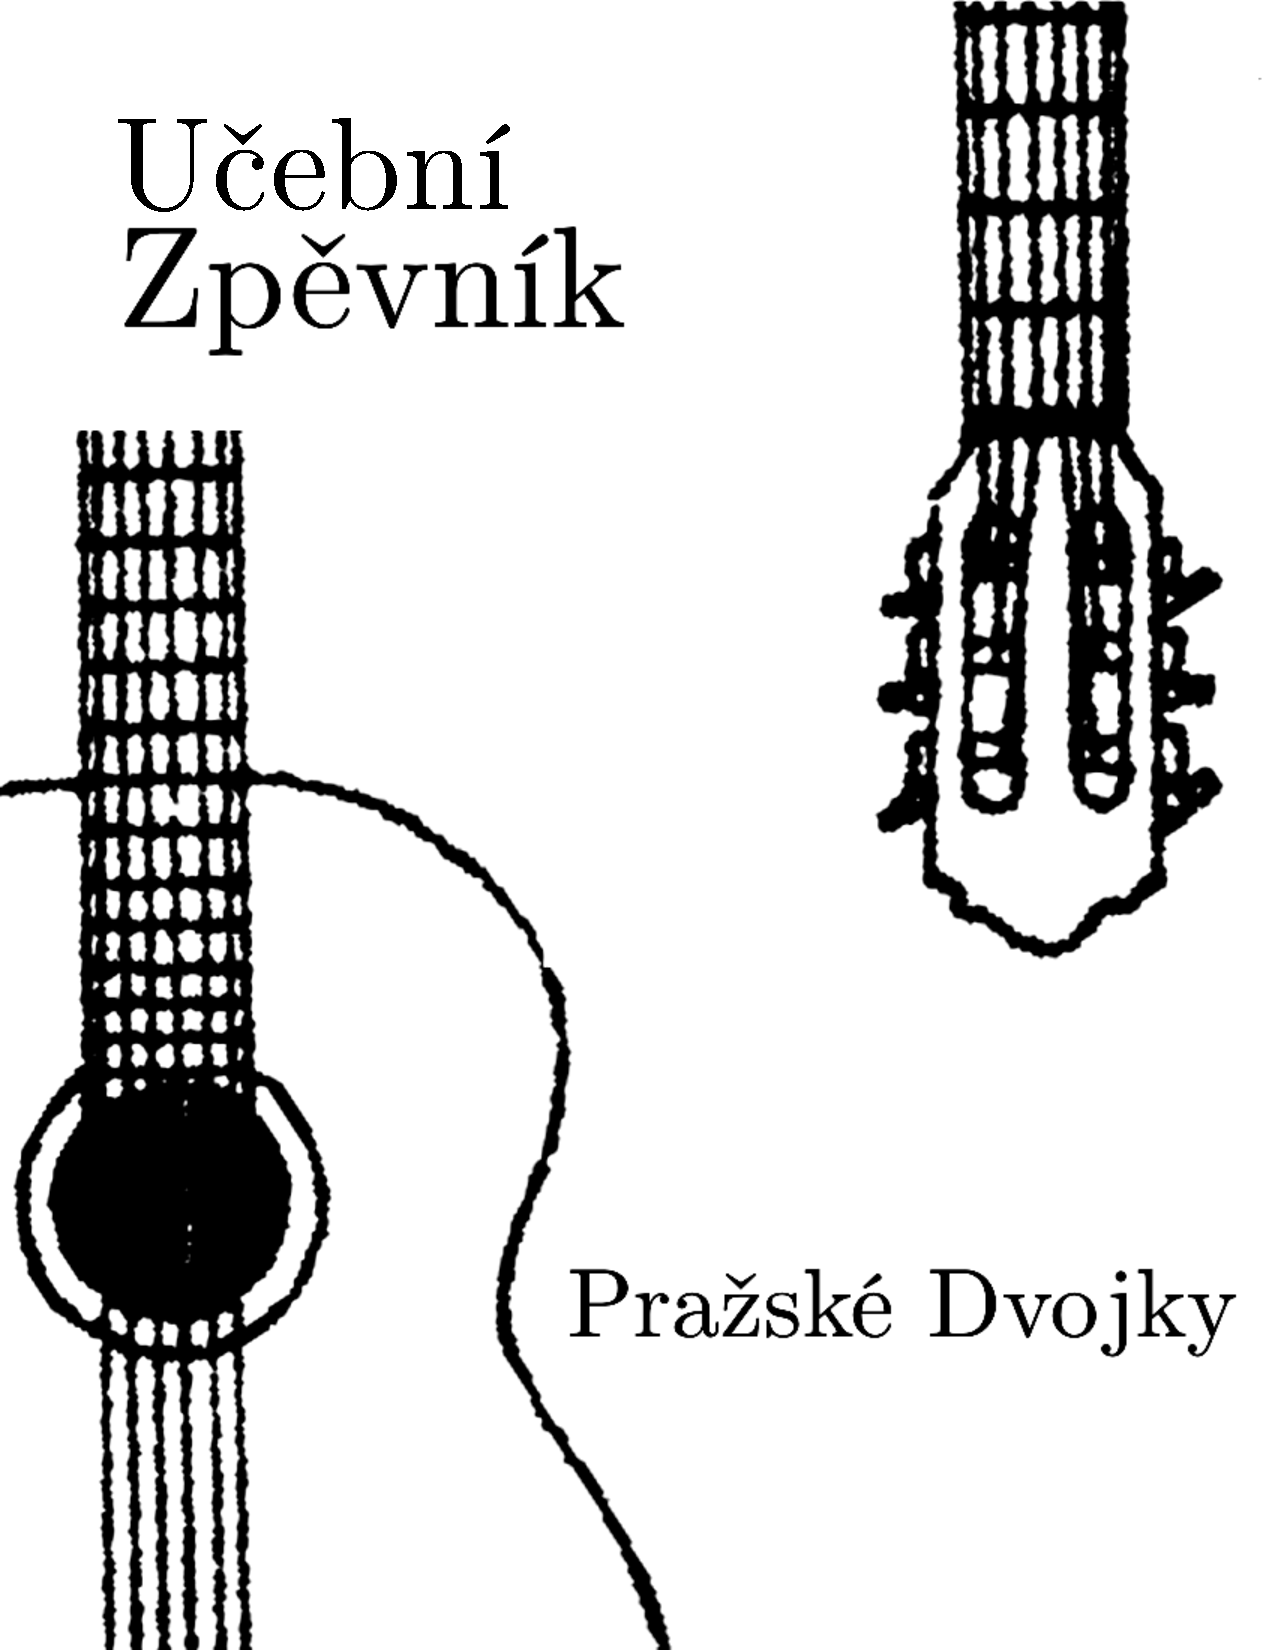
\includepdf{obr/cover}
\newpage
\phantom{prázdná strana}
\newpage

%%%%%%%%%%%% Úvod %%%%%%%%%%%%%%%%%%
\vspace*{4\baselineskip}
\begin{abstract}
\large 

\sffamily
% PŘEDMLUVA
\lettrine{T}{ento} zpěvník slouží jako pomůcka pro učící se kytaristy, aby se
naučili hrát na kytaru. Najdete v něm sice méně písniček, za to však jsou
u~většiny písniček akordy nad celým textem a na konci přehled použitých akordů.
Písničky v tomto zpěvníku obsažené považujeme za vhodné k~učení se hraní na
kytaru.\\
Připomínky uvítáme na emailu \verb|jd@mamlasinky.com|. Kód zpěvníku najdete
i~na GitHubu. Pozn.: abecední pořadí ve zpěvníku nebylo dodrženo,
abyste při hraní vícestranných písniček nemuseli otáčet sránku. \\ \\
%Za úvodní kresbu na přebalu děkujeme $\mathfrak{P}$štrosovi.
Obrázky akordů
používáme ze stránky \url{https://jguitar.com/}.\\\\\\\\\\
Hodně zábavy při zpěvu přejí tvůrci zpěvníku\\\\
$\mathfrak{J}$indra \& $\mathfrak{A}$lbert.\\\\\\\\\\\\\\\\\\\\	
{\tiny \rmfamily Zpěvník 18.09, Bojovná barakuda LTS}
\end{abstract}
\newpage


%%%%%%%%%%%%% Písně %%%%%%%%%%%%%%%%
%% Okraje:
% P+L = 4cm
% T = 1.5cm
% B = 0 cm

\newgeometry{top=1.5cm, bottom=2cm, left=2cm, right=2cm}
\setlrmarginsandblock{1cm}{3cm}{*} %Kvůli dírám pro kroužky
\setulmarginsandblock{1.5cm}{1cm}{*}
\checkandfixthelayout 

%%%%%%%%%%%%% Obsah %%%%%%%%%%%%%%%%
\addtocontents{toc}{\protect\thispagestyle{empty}}
\tableofcontents* \thispagestyle{empty}\newpage
\newgeometry{top=1.5cm, bottom = 0cm, left = 2cm, right = 2cm}
\setlrmarginsandblock{1cm}{3cm}{*} %Kvůli dírám pro kroužky
\setulmarginsandblock{1.5cm}{0cm}{*}
\checkandfixthelayout 



% PRIDAVANI 
\pagestyle{simple}
\phantomsection\addcontentsline{toc}{section}{Anděl}\begin{song}{title=\predtitle \centering Anděl \\\large Karel Kryl   \vspace*{-0.3cm}}  %% sem se napíše jméno songu a autor
\begin{centerjustified}
\nejnejvetsi
\sloka 
	^{G}Z ^{\z Emi}rozmlácenýho kostela ^{G\z}v~krabici ^{D7\z}s~kusem mýdla

	^{G\z}přinesl ^{Emi}jsem si anděla, ^{G\z D7}polámali mu křídla.

	Díval se na mě oddaně, já měl jsem trochu trému,

	tak vtiskl jsem mu do dlaně lahvičku od parfému.

\refren
	^{G\z}A~proto, ^{Emi\z }prosím, věř mi, ^{G\z}chtěl jsem ho ^{D7\z}žádat,
	
	^{G}aby mi ^{Emi\z }mezi dveřmi ^*{G}po mohl ^*{D7}hád at,

	^{G}co mě čeká ^{Emi} ^{D}a nemine, ^{G}co mě čeká ^{Emi} ^{D7}a  ^*{\z G}nemine .

\sloka
	Pak hlídali jsme oblohu, pozorujíce ptáky,
	
	debatujíce o Bohu a hraní na vojáky.

	Do tváře jsem mu neviděl, pokoušel se ji schovat,

	to asi ptákům záviděl, že mohou poletovat.

\refren

\sloka
	Když novinky mi sděloval u okna do ložnice,

	já křídla jsem mu ukoval z mosazný nábojnice,
	
	a tak jsem pozbyl anděla, on oknem odletěl mi,

	však přítel prý mi udělá novýho z mojí helmy.

\refren

\end{centerjustified}
\setcounter{Slokočet}{0}
\end{song}
\newpage
\phantomsection\addcontentsline{toc}{section}{Cestou do Jenkovic}\begin{song}{title=\predtitle\centering Cestou do Jenkovic \\\large Radůza  \vspace*{-0.3cm}}  %% sem se napíše jméno songu a autor
\begin{centerjustified}
\nejnejvetsi
\sloka 
	^{D}Můj děda z kola ^{Hmi\z }seskočil, ^{C\z }před prázdnou kašnou ^{A}na náměstí.
	
	^{D}Na lavičce chleba ^{Hmi\z }posvačil, ^{C\z }seřídil hodinky ^{A}na zápěstí.

\refren /: ^{D\z}A~čápi z komína ^{A}od cihelny, zobákem ^{C\z }klapou, asi jsou ^{G\z }nesmrtelný. :/

\sloka 
	Tři kluci v bílejch košilích dělili se vo poslední spartu,

	ze zídky do záhonu skočili, přeběhli ulici a zmizeli v parku.

\refren

\sloka
	Ve voknech svítěj peřiny, na bílý kafe mlíko se vaří,

	teď právě začaly prázdniny, venku je teplo a všechno se daří.

\refren



\end{centerjustified}
\setcounter{Slokočet}{0}
\end{song}


\begin{figure}[h]
\predtitle\centering
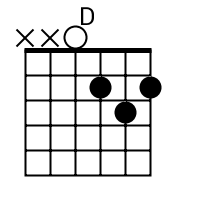
\includegraphics[width=3cm]{../Akordy/d.png}
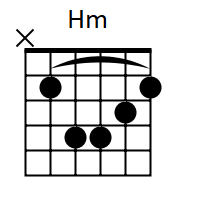
\includegraphics[width=3cm]{../Akordy/hm.png}
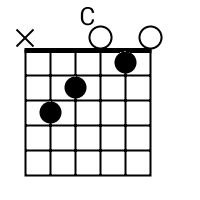
\includegraphics[width=3cm]{../Akordy/c.png}
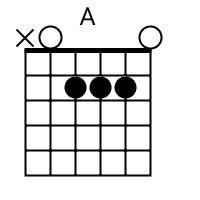
\includegraphics[width=3cm]{../Akordy/a.png}
\end{figure}
\newpage
\phantomsection\addcontentsline{toc}{section}{Dezolát}\begin{song}{title=\centering Dezolát\\\normalsize Vypsaná Fixa \vspace*{-0.3cm}}  %% sem se napíše jméno songu a autor
\moveright 2cm \vbox{      %Varianta č. 1  ---> Jeden sloupec zarovnaný na střed	
\begin{minipage}[t]{0.48\textwidth}\setlength{\parindent}{0.45cm}  %Varianta č. 2 --> Dva sloupce

\sloka
	^{Emi}Ty jsi pěkný ^{\,\,C}dezolát,
	
	^{D{\color{white}\_}}řekla ,,Halí ^{A}Belí''
	
	a byla to pohoda,
	
	třeba se to povede, 
	
	vytáhnem tvý múzy 
	
	a hodíme je za tebe 
	
	a kdo ty múzy zachytí, 

	ten bude mít záruku 
	
	opravdový kvality.
	
	Ty jsi pěkný dezolát.
	
	Tohle řekla ona, 
	
	musíme tě sledovat.
	
\refren
	^{C}A celý ^{Emi}prostor 
	
	je sledovaný
	
	^{C}příjemnými lidmi, kteří olizují 
	
	^{C}šťávu ^{Emi}tekoucí 
	
	z konečků ^{D}prstů.
	
\sloka
	Ty jsi pěkný dezolát.
	
	Ve sprchovým koutě 
	
	teče voda ledová.
	
	Třeba se to povede,
	
	opláchnu svý múzy 
	
	a vypustím je pod sebe. 
	
	Kdo ty múzy zachytí, 
	
	ten bude mít záruku 
	
	opravdový kvality. 
	
	Ty jsi pěkný dezolát. 
	
	Tohle řekla ona.
	
\refren
	
      \end{minipage}\begin{minipage}[t]{0.48\textwidth}\setlength{\parindent}{0.45cm}%\vspace*{0.55cm}  % V případě varianty č.2 jde odsud text do pravé části

\refren
	^{Emi{\color{white}\_\_}}Pustíme si ^{C{\color{white}\_}}starý gramofon, 
	
	^{D{\color{white}\_\_\_\_\_\_\_}}budeme mít ^{A{\color{white}\_}}světy, 
	
	který nás zajímají.
	
	Vinylový bůh je šampion,
	
	proležíme v posteli 
	
	celou neděli.
	
	Pustíme si starý gramofón,
	
	budeme mít světy,
	
	který nás zajímají.
	
	Viny loví bůh, je šampion,
	
	venku ten náš svět 
	
	sledují kamery.
	
	\phantom{h}
	
	A hudba hraje dál\dots
	
	\phantom{h}	
	
	Pustíme si starý gramofon,
	
	budeme mít světy, 
	
	který nás zajímají.
	
	Vinylový bůh je šampion,
	
	venku ten náš svět 
	
	sledují kamery.
	
	\phantom{j}
	
	^{Emi}Jsem z ^{C}toho celej ^{A}žhavej.
	
	
\end{minipage}
}
\setcounter{Slokočet}{0}
\end{song}



\newpage
\phantomsection\addcontentsline{toc}{section}{Hercegovina}\begin{song}{title=\centering Hercegovina \\\normalsize \vspace*{-0.3cm}}  %% sem se napíše jméno songu a autor
\moveright 3.7cm \vbox{      %Varianta č. 1  ---> Jeden sloupec zarovnaný na střed	

\sloka 
	/: ^{G{\color{white}\_\_\_\_\_\_\_\_\_}}Hercegovina, cha-cha-cha-ju-cha-cha,
	
	^{D\,\,}lautr rovina, cha-cha-cha-ju-cha-cha, :/
	
	/: ^{G}tu musela ^{C{\color{white}\_\_\_\_\_\_}}vybojovat ^{D{\color{white}\_\_\_\_\_\_}G}infanteria, cha-cha. :/
	
\sloka
	/: Infanteria, cha-cha-cha-ju-cha-cha,
	
	čestná setnina, cha-cha-cha-ju-cha-cha, :/
	
	/: ta musela bojovati za císaře pána, cha-cha. :/
	
\sloka
	/: Za císaře pána, cha-cha-cha-ju-cha-cha,
	
	a jeho rodinu, cha-cha-cha-ju-cha-cha :/
	
	/: museli jsme vybojovat Hercegovinu, cha-cha. :/
	
\sloka
	/: Vzhůru po stráni, š š š š š,
	
	šnelcuk uhání, š š š š š, :/
	
	/: a pod strání jsou schováni Mohamedáni, cha-cha. :/
	
\sloka
	/: Mohamedáni, cha-cha-cha-ju-cha-cha,
	
	to jsou pohani, cha-cha-cha-ju-cha-cha, :/
	
	/: kalhoty maj roztrhaný a smrkaj do dlaní, cha-cha. :/
	
\sloka
	/: Tyhle Turkyňe, cha-cha-cha-ju-cha-cha,
	
	tlustý jak dýně, cha-cha-cha-ju-cha-cha. :/
	
	/: Císař pan je nerad vidí ve svý rodině, cha-cha. :/
	
\sloka
	/: Tuto píseň skládal, cha-cha-cha-ju-cha-cha,
	
	jeden hoch mladý, cha-cha-cha-ju-cha-cha, :/
	
	/: který se dal skrz svou holku k infanterii, cha-cha. :/
	

}
\setcounter{Slokočet}{0}
\end{song}
\newpage
\phantomsection\addcontentsline{toc}{section}{Kamarádi}%\documentclass[../main.tex]{subfiles}

\begin{song}{title=\centering Kamarádi \\\normalsize Poslední výstřel  \vspace*{-0.3cm}}  %% sem se napíše jméno songu a autor
\moveright \stred \vbox{      %Varianta č. 1  ---> Jeden sloupec zarovnaný na střed


\sloka
	^{Emi}Bývaly chvíle, kdy jsem ^{G}chtěl  sundat 
 
	brýle a ^{Ami}říct ti: ,,Pojď ^{C}ven.``

	Pak jsem to ale nějak překousl, 

	ač jsi mě rozhněval hodně.

\sloka
	Bývaly chvíle, kdy mi nebylo milé, 

	že patřím k takovým lidem. 

	Ne, ne, kámoše si nevybereš, 

	kámoš je ten, kdo na tebe zbyde.

\refren
	Pořád jsme kamarádi, pořád jsme kamarádi.

	Pořád jsme kamarádi, pořád jsme kamarádi.

	Co jsme si, to jsme si, co jsme si, to jsme si 

	pořád jsme kamarádi.

	Co jsme si, to jsme si, co jsme si, to jsme si,

	pořád jsme kamarádi.

\sloka
	Bývaly chvíle, kdy sis chtěl sundat 

	brýle a říct mi: \uv{Pojď ven}. 

	Pak jsi to ale nějak překousl,

	ač jsem tě rozhněval notně.

\sloka
	Bývaly chvíle kdy ti nebylo milé,

	že patříš k takovým lidem.

	Kámoše si prostě nevybereš,

	kámoš je ten kdo na tebe zbyde.

\refren

}
\setcounter{Slokočet}{0}

\end{song}

\newpage
\phantomsection\addcontentsline{toc}{section}{Hey Ho}\begin{song}{title=\predtitle\centering Hey Ho Nobody's Home \vspace*{-0.3cm}}  %% sem se napíše jméno songu a autor
\begin{centerjustified}
\nejnejvetsi
	
\sloka
^{Ami}Hey ^{Emi}ho, ^{Ami}nobody's ^{Emi}home, 

^{Ami}Meat nor ^{Emi}drink nor ^{Ami}money have I ^{Emi}none. Yet 

^{Ami}Every ^{Emi}time I ^{Ami}will be ^{Emi}happy. 

/: ^{Ami}Zum gali ^{Emi}gali gali, ^{Ami}zum gali ^{Emi}gali. :/

\end{centerjustified}
\setcounter{Slokočet}{0}
\end{song}

\begin{figure}[h]
\predtitle\centering
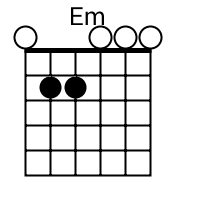
\includegraphics[width=3cm]{../Akordy/em.png}
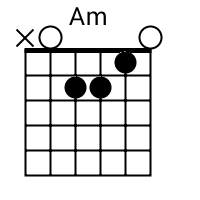
\includegraphics[width=3cm]{../Akordy/am.png}
\end{figure}
\newpage
\phantomsection\addcontentsline{toc}{section}{Knockin' on Heaven's Door}%\documentclass[../main.tex]{subfiles}


\begin{song}{title=\centering Knockin' On Heaven's Door \\\normalsize Bob Dylan  \vspace*{-0.3cm}}  %% sem se napíše jméno songu a autor
\moveright 4.5cm \vbox{      %Varianta č. 1  ---> Jeden sloupec zarovnaný na střed

\sloka
	^{G}Mama, ^{D}take this badge off of me ^{Ami} 
 
	^{G}I can't ^{D}use it ^{C}anymore. 
 
	It's gettin' dark, too dark for me to see.

	I feel like I'm knockin' on heaven's door.

\refren
	^{G}Knock, knock, ^{D}knockin' on heaven's  ^{Ami}door.

	^{G}Knock, knock, ^{D}knockin' on heaven's  ^{C}door. 
 
	Knock, knock, knockin' on heaven's door.

	Knock, knock, knockin' on heaven's door.

\sloka
	Mama, put my guns in the ground 

	I can't shoot them anymore. 

	That long black cloud is comin' down. 

	I feel like I'm knockin' on heaven's door. 

\refren

}
\setcounter{Slokočet}{0}
\end{song}
\begin{figure}[h]
\centering
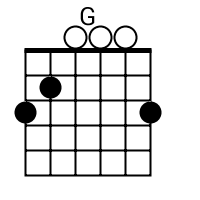
\includegraphics[width=3cm]{../Akordy/g}
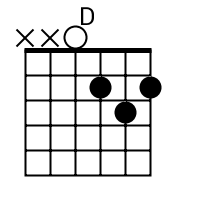
\includegraphics[width=3cm]{../Akordy/d}
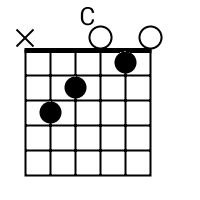
\includegraphics[width=3cm]{../Akordy/c}
\includegraphics[width=3cm]{../Akordy/Am}
\end{figure}
\newpage
\phantomsection\addcontentsline{toc}{section}{Ráda se miluje}%\documentclass[../main.tex]{subfiles}

\begin{song}{title=\centering Ráda se miluje \\\normalsize Karel Plíhal  \vspace*{-0.3cm}}  %% sem se napíše jméno songu a autor
\moveright 4cm \vbox{      %Varianta č. 1  ---> Jeden sloupec zarovnaný na střed	

\refren
^{Hmi}Ráda se miluje, ^{A{\color{white}\_}}ráda ^{D}jí,

^{G{\color{white}\_}}ráda si ^{F#mi\,}jenom tak ^{Hmi{\color{white}\_}}zpívá, 

vrabci se na plotě ^{A\,{\color{white}\_}D\,}hádají, 

^{G{\color{white}\_\_}}kolik že ^{F#mi}času jí ^{Hmi{\color{white}\_}}zbývá.

\sloka
^{G}Než vítr dostrká k ^{D\,{\color{white}\_}}útesu ^{G}tu její legrační ^{{\color{white}\_}D\,\,F#mi}bárku 

a ^{Hmi\,\,}Pámbu si ve svým ^{A{\color{white}\_}D}notesu ^{G{\color{white}\_\_}}udělá ^{F#mi}jen další ^{Hmi\,\,}čárku.

\refren

\sloka
Psáno je v nebeské režii, a to hned na první stránce, 

že naše duše nás přežijí v jinačí tělesný schránce. 

\refren

\sloka
Úplně na konci paseky, tam, kde se ozvěna tříští, 

sedí šnek ve snacku pro šneky -- snad její podoba příští. 


\refren

}
\setcounter{Slokočet}{0}
\end{song}

\newpage
\phantomsection\addcontentsline{toc}{section}{Slavíci z Madridu}%\documentclass[../main.tex]{subfiles}

\begin{song}{title=\centering Slavíci z Madridu \\\normalsize Waldemar Matuška \vspace*{-0.3cm}}  %% sem se napíše jméno songu a autor
\moveright 4.5cm \vbox{      %Varianta č. 1  ---> Jeden sloupec zarovnaný na střed	

\sloka
^{Ami}Nebe je ^{E}modrý a zlatý, ^{Ami}bílá sluneční záře,

horko a ^{E}sváteční šaty, ^{Ami}vřava a zpocený tváře,

vím, co ^{E}se bude dít, býk už ^{Ami}se v ohradě vzpíná,

kdo chce, ^{E}ten může jít, já ^{Ami}si dám sklenici vína.

\refren
^{Dmi}Žízeň je ^{Ami}veliká, život mi utíká,

^{E}nechte mě ^{Ami}příjemně snít,

^{Dmi}ve stínu pod ^{Ami}fíky poslouchat slavíky

^{E}zpívat si s ^{Ami}nima a pít.

\sloka
Ženy jsou krásný a cudný, mnohá se ve mně zhlídla,

oči jako dvě studny, vlasy jak havraní křídla,

dobře vím, co znamená pád do nástrah dívčího klína,

někdo má pletky rád, já si dám sklenici vína.

\refren

\sloka
Nebe je modrý a zlatý, ženy krásný a cudný,

mantily, sváteční šaty, oči jako dvě studny,

zmoudřel jsem stranou od lidí, jsem jak ta zahrada stinná,

kdo chce, ať mi závidí, já si dám sklenici vína.

\refren

}
\setcounter{Slokočet}{0}

\end{song}
\begin{figure}[h]
\centering
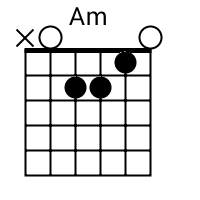
\includegraphics[scale=1.5]{../Akordy/am}
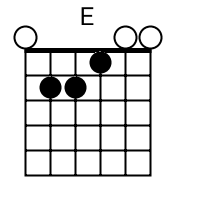
\includegraphics[scale=1.5]{../Akordy/e}
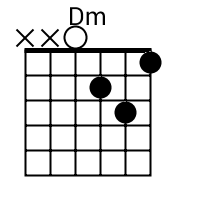
\includegraphics[scale=1.5]{../Akordy/dm}
\end{figure}

\newpage
\phantomsection\addcontentsline{toc}{section}{Zatači}\begin{song}{title=\centering Zatanči \\\normalsize Jaromír Nohavica  \vspace*{-0.3cm}}  %% sem se napíše jméno songu a autor
\moveright \stred \vbox{      %Varianta č. 1  ---> Jeden sloupec zarovnaný na střed	

\sloka
^{Emi G}Zatanči, má milá, ^{D{\color{white}\_\_}}zatanči ^{Emi}pro mé oči,

^{{\color{white}\_\_}G}zatanči a vetkni nůž ^{D}do mých ^{Emi}zad.

Ať tvůj ^{G}šat, má milá, ať ^{D}tvůj šat ^{Emi}na zemi skončí,

ať tvůj ^{G}šat, má milá, ^{D}rázem je ^{Emi}sňat.

\refren
^{Emi G}Zatanči, jako se ^{D{\color{white}\_}}okolo ^{Emi\,\,}ohně tančí,

^{{\color{white}\_\_}G}zatanči jako ^{D{\color{white}\_\_}}na\,\,vodě ^{Emi}loď,

^{{\color{white}\_\_}G}zatanči jako to ^{D}slunce ^{Emi}mezi pomeranči,

^{{\color{white}\_\_}G}zatanči, a ^{D}pak ke mně ^{Emi}pojď.

\phantom{.}

\textbf{Mezihra}

\sloka
Polož dlaň, má milá, polož dlaň na má prsa,

polož dlaň nestoudně na moji hruď.

Obejmi, má milá, obejmi moje bedra,

obejmi je pevně a mojí buď.

\refren

\phantom{.}

\textbf{Mezihra}

\sloka
Nový den než začne, má milá, nežli začne,

nový den než začne, nasyť můj hlad.

Zatanči, má milá, pro moje oči lačné,

zatanči a já budu ti hrát.

\refren

\refren
}
\setcounter{Slokočet}{0}
\end{song}
\newpage
\phantomsection\addcontentsline{toc}{section}{Zabili}\begin{song}{title=\centering Zabili \\\normalsize z filmu Balada pro Banditu  \vspace*{-0.3cm}}  %% sem se napíše jméno songu a autor
\moveright \stred \vbox{      %Varianta č. 1  ---> Jeden sloupec zarovnaný na střed	

\sloka
   ^{C{\color{white}\_\_\_}}Zabili, ^{F{\color{white}\_\_\_}}zabili ^{Dmi{\color{white}\_\_}}chlapa z ^{\,\,\,\,F}Koločavy,

   řekněte hrobaři, kde je pochovaný.


\refren
   ^{C{\color{white}\_\_}}Bylo tu, není tu, havrani ^{F}na plotu,

   ^{C{\color{white}\_\_\_}}bylo víno v sudě, ^{F\,\,}teď tam voda bude,

   není, ^{C{\color{white}\_\_}}není tu.


\sloka
    Špatně ho zabili, špatně pochovali,
    
   vlci ho pojedli, ptáci rozklovali.


\refren


\sloka
   Vítr ho roznesl po dalekém kraji,
   
   havrani pro něho po poli krákají.


\refren


\sloka
   Kráká starý havran, krákat nepřestane,
   
   dokud v Koločavě živý chlap zůstane.
   
   
\refren

}
\setcounter{Slokočet}{0}
\end{song}
\newpage



\begin{song}{title=\centering Strum patterns \\\normalsize Jak hrát na kytaru pravou rukou \vspace*{-0.3cm}}  %% sem se napíše jméno songu a autor

\newcommand{\up}{$\uparrow$} %Brnknutí dolů
\newcommand{\dn}{$\downarrow$} %Brnknutí nahoru
\newcommand{\x}{$\times$} %Ztlumení strun 
\newcommand{\tu}{\textunderscore} % Nehraní ničeho
\centering
\mezera 

%\setlength{\arrayrulewidth}{.1em}
\renewcommand{\arraystretch}{1.4}
\begin{tabular}{l  l  l}
\hline\hline 
Č. & Jak hrát & Kde se vyskytuje  \\ \hline
1  & \dn \up \dn \up \dn \up & základní styl brnkání, který lze zahrát téměř v~každé situaci\\
2  & \dn \tu \dn \up \dn \tu \dn \tu \dn & např. v~písni Slavíci z Madridu  \\
3  & \dn \tu \tu \tu \dn \tu \dn & např. v~písni Knockin' On Heaven's Door  \\
4  & \dn \x  \up \dn \up \dn & např. v~písni Dezolát \\
5  & \dn \up \dn \tu \dn \up & např. v~písni Cesta do Jenkovic \\
6  & \dn \tu \dn \up \tu \up \dn \up & lze hrát např. v~refrénu Cesty do Jenkovic \\
7  & \dn \tu \dn \tu \dn \up \dn \up & lze hrát např. v~refrénu Cesty do Jenkovic \\
\hline \hline
\end{tabular}



	
\setcounter{Slokočet}{0}
\end{song}


\newpage

\pagestyle{empty}

% Aby byla titulni strana a strana s akordy na coveru



%%%%%%%%%%%%% Přehled akordů %%%%%%%%%%%%%%%%
\newgeometry{top=0cm, bottom = 0cm, left = 0cm, right = 0cm}
\thispagestyle{empty}
\begin{figure}[h]
\centering
% PŘEHLED
{\hspace*{-1.5cm}
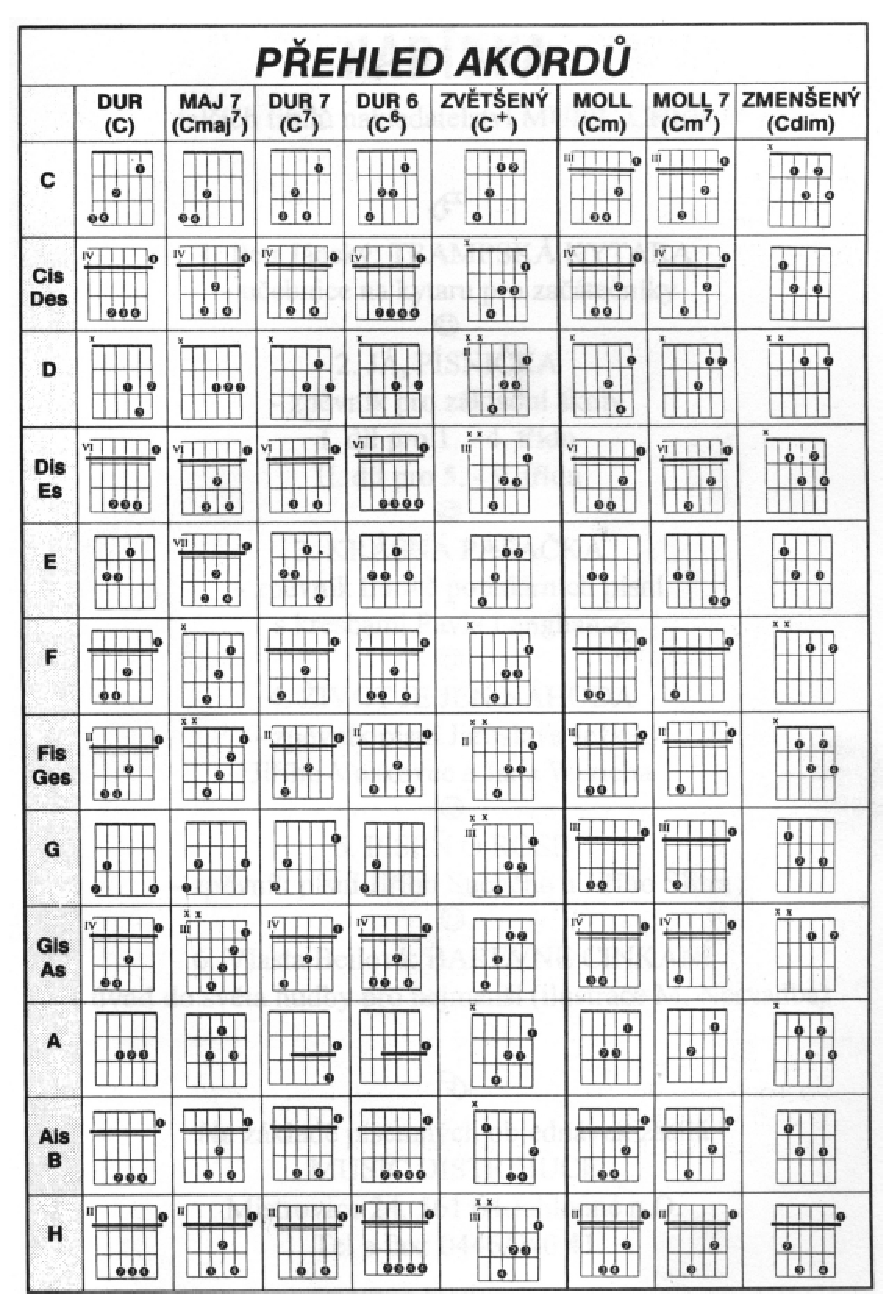
\includegraphics[height=\textheight]{../Akordy/AAAkordy3.pdf}
}
\end{figure}



\end{document}

